%20 min preso!
\documentclass[xcolor=table]{beamer}
\usepackage{beamerthemesplit}
\usepackage{wrapfig}
\usetheme{SPbGU}
\usepackage{pdfpages}
\usepackage{amsmath}
\usepackage{cmap}
\usepackage[T2A]{fontenc}
\usepackage[utf8]{inputenc}
\usepackage[english]{babel}
\usepackage{indentfirst}
\usepackage{amsmath}
\usepackage{tikz}
\usepackage{multirow}
\usepackage[noend]{algpseudocode}
\usepackage{algorithm}
\usepackage{algorithmicx}
\usepackage{fancyvrb}
\usepackage{verbatim}
\usetikzlibrary{calc}
\usetikzlibrary{shapes,arrows}
\usetikzlibrary{arrows,automata}
\usetikzlibrary{positioning}

\usepackage{tabularx}
\newcolumntype{Y}{>{\raggedleft\arraybackslash}X}

\renewcommand{\thealgorithm}{}

\newtheorem{mytheorem}{Theorem}
\renewcommand{\thealgorithm}{}

\newcommand{\tikzmark}[1]{\tikz[overlay,remember picture] \node (#1) {};}
\def\Put(#1,#2)#3{\leavevmode\makebox(0,0){\put(#1,#2){#3}}}

\newcommand{\ltz}{$< 1$}


\tikzset{
    state/.style={
           rectangle,
           rounded corners,
           draw=black, very thick,
           minimum height=2em,
           inner sep=2pt,
           text centered,
           },
}

\beamertemplatenavigationsymbolsempty

\title[Formal Grammars + Neural Networks]{On Secondary Structure Analysis by Using
Formal Grammars and Artificial Neural
Networks}
%\subtitle[YaccConstructor]{Parsing techniques for graph analysis}
% То, что в квадратных скобках, отображается в левом нижнем углу.
\institute[]{
JetBrains Research, Programming Languages and Tools Lab  \\
Saint Petersburg University
}

% То, что в квадратных скобках, отображается в левом нижнем углу.
\author[Polina Lunina]{\textbf{Polina Lunina}, Semyon Grigorev}

\date{September 6, 2019}

\begin{document}
{
\begin{frame}[fragile]
  \begin{table}
  \centering
  \begin{tabularx}{\linewidth}{YcX}
    
\includegraphics[height=1.5cm]{pictures/jetbrainsResearch.pdf} \hfill
    & \begin{minipage}[t]{0.3\textwidth}\center \vspace{-1cm}  CIBB 2019
      \end{minipage}
    & \hfill 
\includegraphics[height=1.5cm]{pictures/SPbGU_Logo.png}
  \end{tabularx}
  \end{table}
  \titlepage
\end{frame}
}

\begin{frame} \frametitle{Genomic Sequences Analysis}
\begin{tabular}{cl}  
    \parbox{0.44\linewidth}{
        \begin{itemize}
            \item Problems
            \begin{itemize}
                \item Genomic sequences classification
                \item Subsequences detection
            \end{itemize}
            \item Secondary structure handling
            \item Probability estimation for noisy data processing
        \end{itemize}
    }
    & \begin{tabular}{l}
        \vspace{-0.8cm}
        \hspace{-0.8cm}
        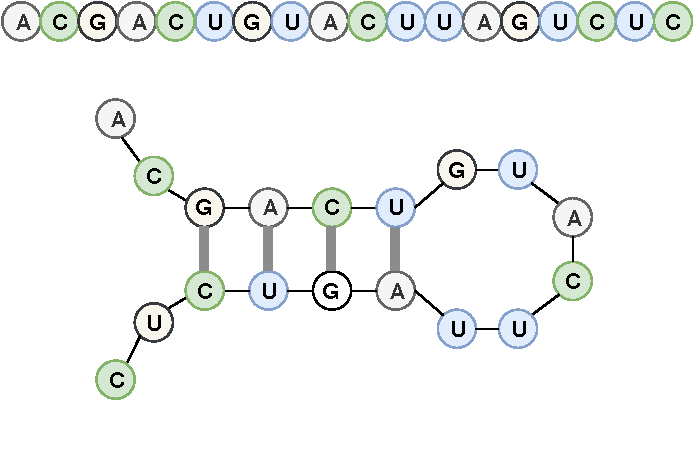
\includegraphics[width=6.5cm]{pictures/molekula.pdf}
    \end{tabular}  \\
\end{tabular}
\end{frame}

\begin{frame} \frametitle{Solution Structure}
\scriptsize
  \begin{tikzpicture}[->,>=stealth']
  \node[state,
        align=left,
        text width = 3.2cm] (grm)
   {
   \textbf{Ordinary Grammar}\\
   Describes the features of secondary structure.
   };

  \node[state,
        below of=grm,
        node distance=1.6cm,
        align = left,
        text width = 3.2cm] (sqs)
   {
   \textbf{Sequences}\\
   Text in the $\{A, C, G, U\}$ alphabet.
   };

  \node[state,
        below right = -0.3cm and 0.6cm of grm,
        align = left,
        text width = 2.7cm](parser)
  {
  \textbf{Parser}\\
  Extracts the features from sequence.
  };

  \node[state,
        right of=parser,
        node distance=4.3cm,
        align = left,
        text width = 4.7cm] (mtrx)
  {
\textbf{Matrices}\\
{\tiny
\[ \left( \begin{array}{cccc}
0 & 1 & 0 & 1\\
0 & 0 & 1 & 0\\
0 & 0 & 0 & 1\\
0 & 0 & 0 & 0
\end{array} \right)\]}
\vspace{-0.2cm}

  Parsing result for a sequence $\omega$ is a boolean matrix~$M$, where $ M[i,j] = 1 $ $\iff \text{\ttfamily{s}} \xrightarrow{*}{} \omega[i,j]$.
  };


  \node[state,
        below of = mtrx,
        node distance=4cm,
        align = left,
        text width = 4.7cm](vector)
  {
  \textbf{Vectors}\\
  \vspace{-0.1cm}

{\tiny
\[ \left( \begin{array}{cccc}
0 & 1 & 0 & 1\\
0 & 0 & 1 & 0\\
0 & 0 & 0 & 1\\
0 & 0 & 0 & 0
\end{array} \right)\]}
\vspace{-0.45cm}
$$\Downarrow$$
\vspace{-0.6cm}
$$\texttt{[0,1,0,1,0,1,0,0,1,0]}$$
\vspace{-0.6cm}
$$\Downarrow$$
\vspace{-0.6cm}
$$\texttt{[84,128]}$$

\vspace{-0.25cm}
  Line-by-line compressed matrix representation. Bottom left triangle is empty, so, can be ignored.
  };

  \node[state,
        below left = -4cm and 0.5cm of vector,
        align = left,
        text width = 4.7cm](DNN)
  {
  \textbf{Neural Network}\\

  Dense neural network with aggressive dropout and batch normalization for learning process stabilization.
  \\
  \vspace{-0.3cm}
  \begin{center}
  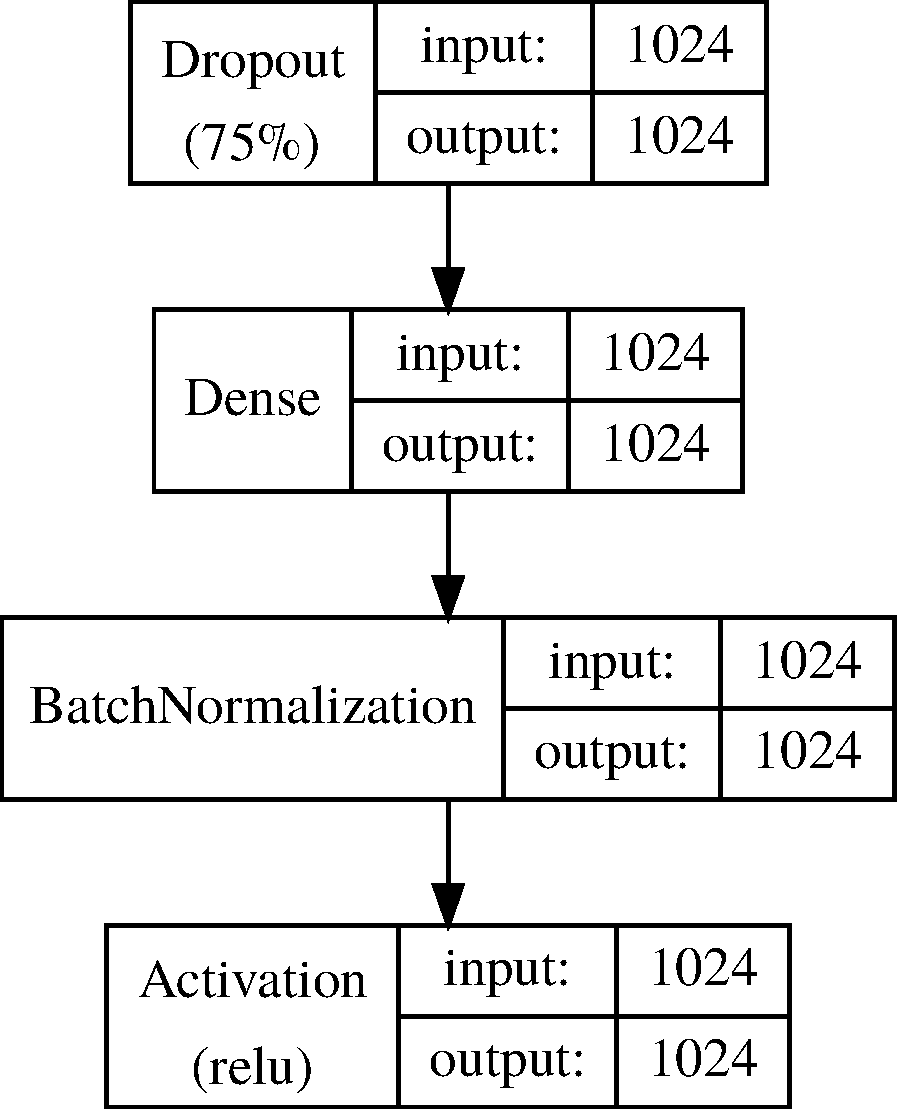
\includegraphics[width=2.5cm]{pictures/bb.pdf}
  \end{center}

  };
  
    \node[state,
        left of = DNN,
        node distance=3.7cm,
        align = left,
        text width = 1cm](result)
  {
  \textbf{Result}
  };

  \path (grm.east) edge (parser.-200)
   (sqs.east) edge (parser.-160)
   (parser) edge (mtrx)
   (mtrx) edge (vector)
   (vector) edge (DNN)
   (DNN) edge (result)
   ;

  \end{tikzpicture}

  \tikzmark{zzz}{
  }
  \pause
  \onslide<2>{\tikz[overlay,remember picture]{\draw[draw=red,thick,double,fill opacity=0.2, rounded corners] ($ (zzz) + (0.01,8.20)$) rectangle ($ (zzz) + (3.35,5.52)$);}}

  \onslide<3>{\tikz[overlay,remember picture]{\draw[draw=red,thick,double,fill opacity=0.2, rounded corners] ($ (zzz) + (3.99,7.4)$) rectangle ($ (zzz) + (6.84,6.31)$);}}

  \onslide<4>{\tikz[overlay,remember picture]{\draw[draw=red,thick,double,fill opacity=0.2, rounded corners] ($ (zzz) + (7.3,8.27)$) rectangle ($ (zzz) + (12.15,5.41)$);}}

  \onslide<5>{\tikz[overlay,remember picture]{\draw[draw=red,thick,double,fill opacity=0.2, rounded corners] ($ (zzz) + (7.3,4.67)$) rectangle ($ (zzz) + (12.15,1.03)$);}}

  \onslide<6>{\tikz[overlay,remember picture]{\draw[draw=red,thick,double,fill opacity=0.2, rounded corners] ($ (zzz) + (1.92,5.01)$) rectangle ($ (zzz) + (6.77,0.34)$);}}

  \onslide<7>{\tikz[overlay,remember picture]{\draw[draw=red,thick,double,fill opacity=0.2, rounded corners] ($ (zzz) + (0.06,3.0)$) rectangle ($ (zzz) + (1.21,2.36)$);}}

\end{frame}


\begin{frame}{Example}
\centering
 \texttt{CCCC{\color{red}AUUGCCAAGG}ACCCCA{\color{red}CCUUGGCAAU}CCC}
\vspace{1cm}

\tikzmark{xx}{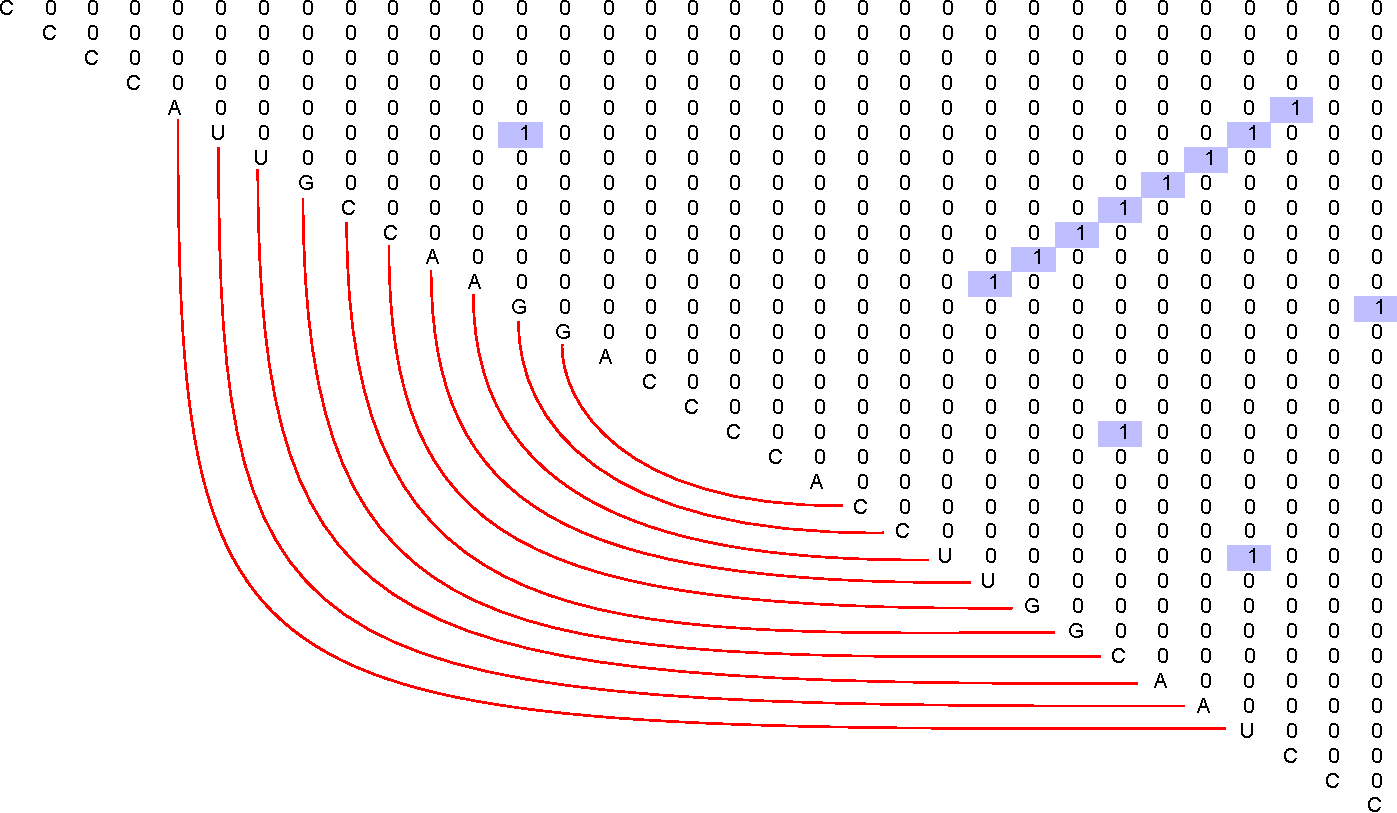
\includegraphics[width=.8\textwidth]{pictures/mtr.pdf}}
\onslide<2-3>{
\tikz[overlay,remember picture]{
\draw[draw=red,thick,fill opacity=0.2] ($(xx) + (1.1,4.97)$) rectangle ($(xx) + (9.05,3.235)$);
}
}

\onslide<3>{
\tikz[overlay,remember picture]{
\draw[draw=red,thick,fill opacity=0.2] ($(xx) + (5.8,4.97)$) rectangle ($(xx) + (8.75,0.4)$);
}
}
\end{frame}


\begin{frame}{Data Locality Preservation}
\textbf{Problem:} data locality is broken during vectorization
\vspace{8pt}

\textbf{Solution:}
    \begin{itemize}
        \item Represent parsing result as an image
        \item Use convolutional layers for such images processing
    \end{itemize}
\end{frame}

\begin{frame}{Parsing Results Representation}
\scriptsize 
  \begin{tikzpicture}[->,>=stealth']

  \node[state,
        align = left,
        text width = 5.5cm] (mtrx)
  {
    \textbf{Matrices}\\
{\tiny
\[ \left( \begin{array}{cccc}
0 & 1 & 0 & 1\\
0 & 0 & 1 & 0\\
0 & 0 & 0 & 1\\
0 & 0 & 0 & 0
\end{array} \right)\]}
    \vspace{-0.1cm}

  Parsing result for sequence $\omega$ is a boolean matrix~$M$, where $ M[i,j] = 1 \iff $ \\ $\text{\ttfamily{s}} \xrightarrow{*}{} \omega[i,j]$.
  };

  \node[state,
        right of=mtrx,
        node distance=6.5cm,
        align = left,
        text width = 5.5cm](vector)
  {
  \textbf{Vectors}\\
  \vspace{-0.1cm}

$$\texttt{[0,1,0,1,0,1,0,0,1,0]}$$
\vspace{-0.6cm}
$$\Downarrow$$
\vspace{-0.6cm}
$$\texttt{[84,128]}$$

\vspace{-0.25cm}
  Line-by-line compressed matrix representation. Bottom left triangle is empty, so, can be ignored. It requires the equal length of the sequences and breaks data locality.
  };

\node[state,
      line width=0.5mm,
      below = 0.8 of mtrx,
      align = left,
      text width = 5.5cm](image)
{
\textbf{Images}\\
\vspace{-0.3cm}
\begin{center}
{\setlength{\fboxsep}{0pt}
 \framebox{%
  
\includegraphics[width=1.5cm]{pictures/bmp.png}}}
\end{center}
\vspace{-0.3cm}
The false bits of the matrix are represented as white pixels and the true bits as black ones. It is possible to process sequences with different lengths and data locality is preserved.

};


  \path 
   (mtrx) edge (vector)
   (mtrx.south) edge (image.north)
   ;

  \end{tikzpicture}
\end{frame}


\begin{frame}{Parsing Elimination}
\textbf{Problem:} parsing is a time-consuming operation
\vspace{8pt}

\textbf{Solution:}
    \begin{itemize}
        \item Create a network which handles original sequences
        \item Use two-staged learning
        \begin{itemize}
            \item Train network on images or vectors for a given problem
            \item Extend it by several input layers that take the nucleotide sequence as an input and convert it to the parsing result 
        \end{itemize}
    \end{itemize}
\end{frame}

\begin{frame}{Neural Networks}
\begin{center}
\vspace{-0.4cm}
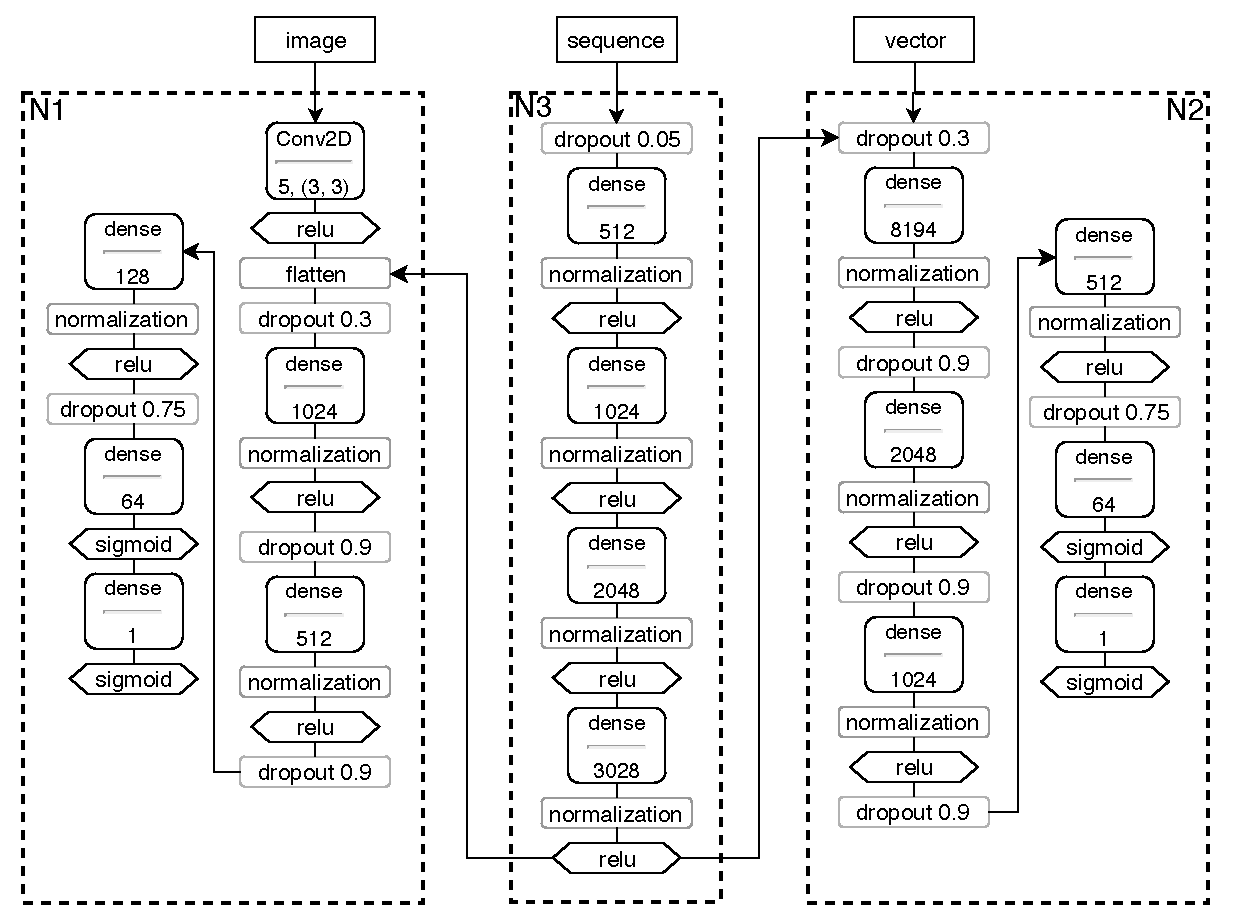
\includegraphics[width=11cm]{pictures/nn_all.pdf}
\end{center}

\tikzmark{zzz}{
}
\pause
\onslide<2>{\tikz[overlay,remember picture]{\draw[draw=red,thick,double,fill opacity=0.2] ($ (zzz) + (0.58,8.1)$) rectangle ($ (zzz) + (4.27,0.84)$);}}

\onslide<3>{\tikz[overlay,remember picture]{\draw[draw=red,thick,double,fill opacity=0.2] ($ (zzz) + (7.74,8.1)$) rectangle ($ (zzz) + (11.44,0.84)$);}}

\onslide<4>{\tikz[overlay,remember picture]{\draw[draw=red,thick,double,fill opacity=0.2] ($ (zzz) + (5.03,8.1)$) rectangle ($ (zzz) + (6.95,0.84)$);}}

\onslide<5>{\tikz[overlay,remember picture]{\draw[draw=red,thick,double,fill opacity=0.2] ($ (zzz) + (0.58,8.1)$) rectangle ($ (zzz) + (6.95,0.84)$);}}

\onslide<6>{\tikz[overlay,remember picture]{\draw[draw=red,thick,double,fill opacity=0.2] ($ (zzz) + (5.03,8.1)$) rectangle ($ (zzz) + (11.44,0.84)$);}}

\end{frame}


\begin{frame}{Evaluation}
\begin{itemize}
    \item tRNA sequences analysis tasks
    \begin{itemize}
        \item Classification into two classes: eukaryotes and prokaryotes
        \item Classification into four classes: archaea, bacteria, plants and fungi
    \end{itemize}
    \item Databases
    \begin{itemize}
        \item tRNADB-CE
        \item Genomic tRNA Database
    \end{itemize}
\end{itemize}
\end{frame}

\begin{frame}{Results}
EP --- eukaryotes/prokaryotes task

ABFP --- archaea/bacteria/plants/fungi task

\begin{table}[h]
\centering
\caption{Base and extended models test results by accuracy metrics}
\begin{tabular}{|l||l|l||l|l|}
\hline
Classifier                                                               & \multicolumn{2}{l||}{EP}               & \multicolumn{2}{l|}{ABFP}           \\ \hline \hline
Approach                                                                 & Vector-based       & Image-based      & Vector-based      & Image-based     \\ \hline
\begin{tabular}[c]{@{}l@{}}Base model\\ accuracy\end{tabular}            & 94.1\%             & 96.2\%           & 86.7\%            & 93.3\%          \\ \hline
\begin{tabular}[c]{@{}l@{}}Extended model \\ accuracy\end{tabular}       & 97.5\%             & 97.8\%           & 96.2\%            & 95.7\%          \\ \hline
\begin{tabular}[c]{@{}l@{}}Total training \\ time\end{tabular}       & 30000s             & 4600s           & 31800s            & 3600s          \\ \hline
\begin{tabular}[c]{@{}l@{}}Samples for\\ train:valid:test\end{tabular} & \multicolumn{2}{l||}{\begin{tabular}[c]{@{}l@{}}20000:5000:10000\\ (57\%:14\%:29\%)\end{tabular}} & \multicolumn{2}{l|}{\begin{tabular}[c]{@{}l@{}}8000:1000:3000\\ (67\%:8\%:25\%)\end{tabular}} \\ \hline
\end{tabular}
\label{acc}
\end{table}

\end{frame}

\begin{frame}{Results}
EP --- eukaryotes/prokaryotes task

ABFP --- archaea/bacteria/plants/fungi task

\begin{table}[h]
\scriptsize
\centering
\begin{tabular}{|l||l|l|l|l|l|}
\hline
\multirow{2}{*}{Classifier} & \multirow{2}{*}{Class} & \multicolumn{2}{l|}{Vector-based approach} & \multicolumn{2}{l|}{Image-based approach} \\ \cline{3-6} 
                            &                        & precision         & recall        & precision        & recall        \\ \hline \hline
\multirow{2}{*}{EP}         & prokaryotic            & 95.8\%            & 99.4\%        & 96.2\%           & 99.4\%        \\ \cline{2-6} 
                            & eukaryotic             & 99.4\%            & 95.6\%        & 99.4\%           & 99.5\%        \\ \hline \hline
\multirow{4}{*}{ABFP}       & archaeal               & 91.1\%            & 99.2\%        & 91.6\%           & 98.5\%        \\ \cline{2-6} 
                            & bacterial              & 96.6\%            & 95.1\%        & 95.2\%           & 95.5\%        \\ \cline{2-6} 
                            & fungi                  & 98.5\%            & 94.9\%        & 97.5\%           & 94.3\%        \\ \cline{2-6} 
                            & plant                  & 99.4\%            & 95.7\%        & 99.2\%           & 94.7\%        \\ \hline
\end{tabular}
\end{table}
\end{frame}

\begin{frame}{Conclusion}
\begin{itemize}
    \item We improved the quality of secondary structure analysis by combination of formal grammars and neural networks 
    \begin{itemize}
        \item Parsing result in a form of image can be handled by convolutional layers and it preserves data locality
        \item The parsing step can be removed from the final pipeline which allows to run models on the original RNA sequences        
    \end{itemize}
    \item The improved version is applicable for real-world problems
\end{itemize}
\end{frame}

\begin{frame}{Future Work}
\begin{itemize}
    \item Deep convolutional networks for secondary structure analysis
    \item Other RNA sequences analysis tasks
    \begin{itemize}
        \item 16s rRNA classification
        \item Chimeric sequences filtration
    \end{itemize}
    \item Secondary structure prediction by generative networks
\end{itemize}

\end{frame}

\begin{frame}
\frametitle{Contact Information}
\begin{itemize}
  \item Semyon Grigorev:
    \begin{itemize}
      \item \href{mailto:s.v.grigoriev@spbu.ru}{s.v.grigoriev@spbu.ru}
      \item \href{mailto:semyon.grigorev@jetbrains.com}{semyon.grigorev@jetbrains.com}
    \end{itemize}
  \item Polina Lunina: \href{mailto:lunina\_polina@mail.ru}{lunina\_polina@mail.ru}
  \item Secondary structure analyzer project: \href{https://research.jetbrains.org/groups/plt\_lab/projects?project\_id=43}{https://research.jetbrains.org/groups/plt\_lab/projects?project\_id=43}
\end{itemize}
\vspace{0.3cm}
\center{\huge{Thanks!}}
\end{frame}
\end{document}
